\documentclass[12pt,a4paper]{report}
\usepackage[frenchb]{babel}
\usepackage[utf8]{inputenc}
\usepackage[export]{adjustbox}
\usepackage{verbatim}
\usepackage{amsmath}
\usepackage{amsfonts}
\usepackage{amssymb}
\usepackage{listings}
\usepackage{graphicx}
\usepackage{pgf, tikz}
	\usetikzlibrary{arrows, shapes, positioning}
\usepackage{hyperref}
\hypersetup{%
    pdfborder = {0 0 0}
}
\author{Maugey Rémy - Bernard Jérémi - De Pourquéry Benjamin - Decoudras Hadrien}
\title{Rapport projet compilation}

\usepackage{tikz}

\begin{document}

\begin{titlepage}
  \begin{sffamily}
  \begin{center}

    % Upper part of the page. The '~' is needed because \\
    % only works if a paragraph has started.
    
\includegraphics[scale=0.05]{logo.jpg}~\\[1.5cm]
    % Author and supervisor
    \begin{minipage}{0.43\textwidth}
      \begin{flushleft} \large
		MAUGEY Rémy\\
		De POURQUERY Benjamin\\
		DECOUDRAS Hadrien\\
		BERNARD Jérémi\\		
		
      \end{flushleft}
    \end{minipage}

	\topskip0pt
	\vspace*{\fill}
	\Huge{Rapport de projet technologique}\\
	\Large{Vison stéréoscopique pour robot}\\
	\vspace*{\fill}

	\vfill
    % Bottom of the page
    {\large \today}

  \end{center}
  \end{sffamily}
\end{titlepage}

\chapter{Introduction}


L'objectif de ce projet est de développer un outil implémenté sur un robot lui permettant de suivre à un mètre une personne grâce à deux caméras.\\\\

Le projet est divisé en deux parties indépendante, effectué sur les deux semestres. 
La première partie a pour but de prendre en main les outils utilisés au cours de l'année, à savoir le langage c++ (à travers qt) et la bibliothèque openCV.
Durant cette première partie sera développé un mini programme de traitement d'images. 

La deuxième partie à pour objectif de programmer le robot et d'effectuer des simulations grâce au logiciel Unity. En effet, comme le robot n'est pas forcement accessible aux membres du groupe, il est préférable de faire appelle à une simulation pour pouvoir tester les algorithmes n'importe quand.\\\\

Qt est une bibliothèque logicielle d'interface graphique, nous utiliserons cet outil pour développer l'interface du logiciel.\\

OpenCV (open computer vision) est un bibliothèque d'algorithmes de traitement d'images, de vidéos et autres. Ici elle sera utilisée pour programmer les fonctions du logiciel en rapport avec les images.\\


%Petite explication de la procédure de comment fonctionne la stereovision ...
\section{Cahier des charges}
Le cahier des charges s'oriente uniquement sur l'objectif du projet, c'est à dire sur la deuxième parties du semestre.
\subsection{Besoin fonctionnels}
	%Identifie une personne
	%Se meut
	%Calcule une distance
	Le logiciel doit prendre en entré deux images au format png représentant les images gauche et droite.
	Grâce à ces images, nous générerons la carte de disparité puis grâce à cette dernière et que caractéristique des caméras, nous pourrons générer la carte de profondeur. C'est à dire que chaque pixel de cette image correspondrons à la distance entre l'objet et les caméras.
	En fonction de cette carte de profondeur, nous serons dans la capacités de faire mouvoir le robot.
	Il sera nécessaire d'avoir une image de référence de la personne à suivre à travers une phase d'initialisation. Dans ce cas, la première image prise par le robot sera considérée comme la référence. Il faut donc que le robot soit bien placé à un mètre de la personne lors de son démarrage et que cette dernière soit la seul dans le cadre des caméras.
\subsection{Besoin non fonctionnels}
	%Robuste aux chagement de luminosité
	%changement de personne
	%chagement d'environnement
	La carte de disparité est fortement liée aux images d'entrées, de ce faite, les changements de luminosité et d'environnement peuvent poser des problèmes à cause notamment de l'utilisation d'une référence.
	Le programme doit donc être robuste à ces différents changement.\\
	Le robot doit être aussi capable de suivre la bonne personne même si une autre personne parasite rentre dans le cadre.
	
\chapter{Implémentation}

\section{Logiciel QT}
%Partie Qt
Le premier semestre c'est orienté autour du développement d'un petit programme de traitement d'image. Le programme affiche une fenêtre ainsi que plusieurs menu, l'un deux permet d'ouvrir un fichier au format png.
Le fichier doit nécessairement contenir les deux images juxtaposées pour que les algorithmes implémenté fonctionnes. On peut ensuite couper l'image en deux, on peut flouté l'image grâce à la méthode "blur" d'OpenCV. On peut aussi appliquer à l'image différent algorithme comme l'algorithme de Sobel, comme présenté sur les figures ci contre.
\begin{center}
\begin{tabular}{cc}
  \vspace{0pt} 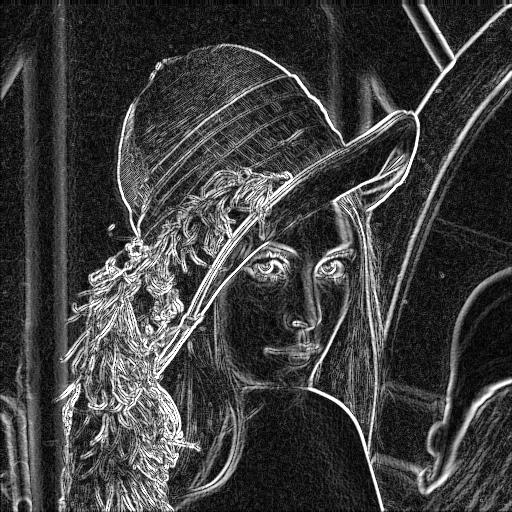
\includegraphics[width=0.49\textwidth]{sobel.jpg} &
  \vspace{0pt} 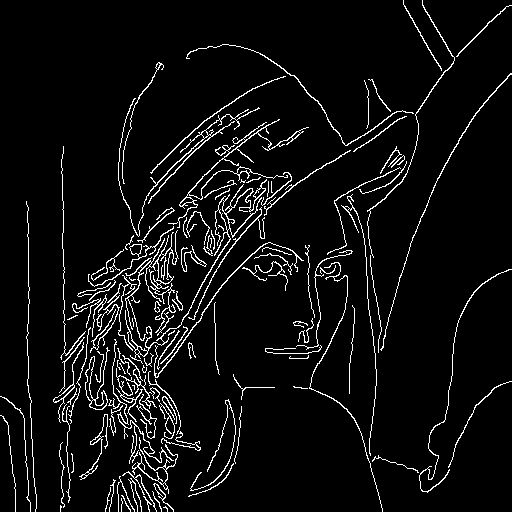
\includegraphics[width=0.49\textwidth]{canny.jpg} \\
    
  Figure 2.1.1 Sobel & Figure 2.2.2 Canny
\end{tabular}
\end{center}

Ces différentes méthodes on été implémentées dans le but de comprendre comment opencv fonctionnait, ainsi que de développer et de tester une première esquisse des fonctions que nous utiliserons dans le robot.

Il a fallu créer des méthodes de conversion d'images entre les images de qt et les images de opencv. Deux méthodes ont donc été développées,

\begin{lstlisting}{Language=C++}
cv::Mat ImageTools::imageToMat(QImage const& src);
QImage ImageTools::cvMatToImage(const cv::Mat& inMat);
\end{lstlisting}

Toutes les méthodes en rapport avec le traitement d'image ont été implémentées dans la classe \textit{imagetools}. Au début, nous conservions les images sous forme de QImage ce qui nous obligeais à convertir à chaque fois. On a fini par réécrire le programme avec des matrices opencv en images membre et la classe \textit{imagetools} sous forme d'un singleton, simplifiant le code.\\
Le logiciel permet aussi de faire de la reconnaissance de paternes grâce aux algorithmes de \textit{flann} et de surf. Cependant ce dernier n'est pas open source donc la méthode \textit{flann} est implémenté mais n'est pas forcement proposé à l'utilisateur final.\\
Enfin, le logiciel permet de créer une carte de disparité grâce à l'algorithme \textit{stereosgbm} ou à l'algorithme \textit{stereobm}.\\

Cette partie nous à permis de prendre en main le c++ ainsi que la bibliothèque opencv. 

Grâce à ce petit outil, nous avons tester les deux algorithmes permettant de générer des cartes de disparité. Nous avons ainsi retenu \textit{stereosgbm} qui est plus performant et plus simple à utiliser. Cela nous à permis de choisir des paramètres de \textit{stereosgbm} jugés bon.

\section{Simulation et test}
%partie Unity
Durant le second semestre, l'objectif était d'implémenter les algorithmes précédent pour les utiliser sur le robot. Le but est de créer une carte de profondeur grâce aux images du robot pour lui permettre de ce déplacer en fonction de la personne.\\
Comme nous n'avons forcement pas accès au robot, nous avons décidé de faire une simulation simple sur le logiciel Unity.\\
Unity fonction grâce à des scripts écrit en c\#, un langage de programmation de haut niveau créé à la base par Microsoft mais qui dans ce cas est utilisé en temps que script grâce à son implémentation libre Mono. Le c\# a une syntaxe proche de celle du java.\\\\

Unity permet de créer des scènes 3D, nous avons aussi utilisés le magasin d'objets intégré pour notre personnage. Nous pouvons ensuite ajouter des caméras et attacher des scripts au différents objets.\\
Voici ci-contre le résultat obtenu.

	\begin{center}
		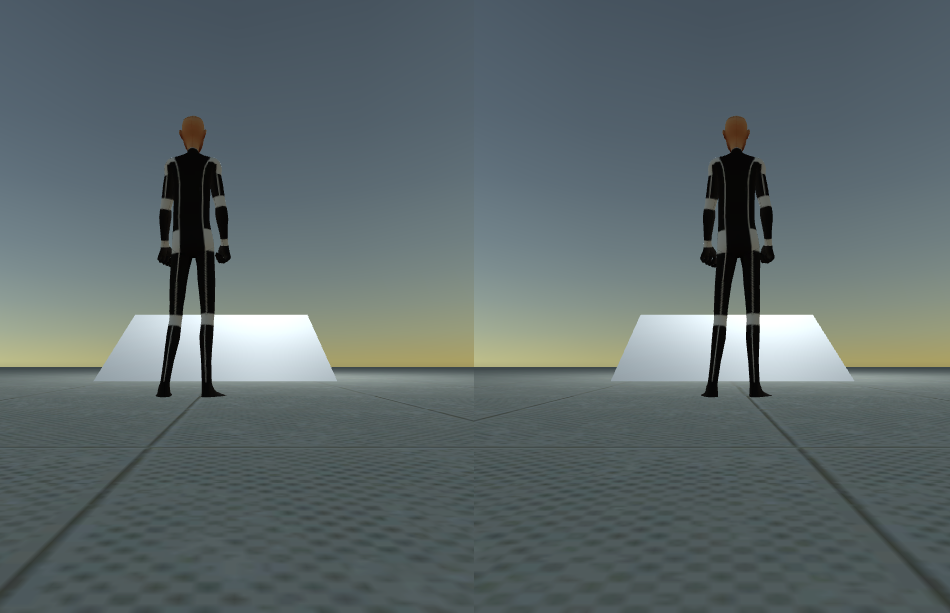
\includegraphics[scale=0.5]{Screenshot_skybox.png}
		Figure 2.3.1 Image issue de Unity\\
	\end{center}
 	
\paragraph{Problèmes rencontrés}
Le logiciel est performant pour créer des petites scènes 3d mais il est très difficilement intégrable dans git ce qui pose des problèmes pour travailler simultanément sur la simulation.

\section{Création de la bibliothèque}
Pour faire la transition entre les algorithmes, l'implémentation du robot et la simulation nous avons décidé de faire une bibliothèque externe contenant tous le code.
Cette bibliothèque a pour tâche d'être utilisée comme simple fichier objet dans le robot, relié grâce à l'édition des liens. Mais elle a aussi pour tâche d'être compilée sous forme d'une bibliothèque partagée (.so) et chargée dans Unity. Les scripts c\# d'Unity se charge juste d'appeler les fonctions c++.

Voici ci-dessous une représentation des interactions entre Unity et la bibliothèque.
\begin{center}
\begin{tikzpicture}
  	\node[draw] (camera) 	at (0, 0) 	{caméras};
  	\node[draw] (conv) 		at (0, -2) 	{Conversion vers une structure Opencv};
	\node[draw] (disp) 		at (0, -4) 	{Calcul de la carte de disparité};
	\node[draw] (depth)		at (0, -6)	{Calcul de la carte de profondeur};
  

 	\draw[->] (camera) to (conv);
 	\draw[->] (conv) to (disp);
 	\draw[->] (disp) to (depth);
 	
 	%partie droite
	 	
	\draw (5,-2) to (5.5, -2);
	\draw (5.5,-2) to (5.5, -6);
	\draw (5,-6) to (5.5,-6);
	\draw (5.5,-4) to (6,-4);
   	\node (dll)		at (7, -4.05)	{Code c++};
   	
	\draw (5, 0) to (6, 0);
	\node (script)	at (7, 0) {Script c\#,};
	\node at (8.2, -0.5) {GetNativeTexturePtr();};
		
	\draw[<-] (camera) to (-3.5, 0);
	\draw (depth) to (-3.5, -6);
	\draw (-3.5, -6) to[in=180, out=180] (-3.5, 0);

	\node[fill=white]	(update)	at (-5.2,-3) {update()};
	
\end{tikzpicture}

Figure 2.3.2 Interaction entre Unity et la bibliothèque.

\end{center}
\paragraph{Problèmes rencontrés}
Des problèmes ont été rencontrés lors de l'utilisation de la bibliothèque sous Unity. Ce dernier plantait quelque fois de manière obscure. (Sûrement due à la version très précoce sous linux) Cependant l'intégration dans Unity n'est pas exclue.

\paragraph{Solutions envisagés}
Nous avons décidé de créer en parallèle de l'intégration à Unity un automate écrit en c++ permettant de tester les algorithmes. Un script c\# se charge de prendre une capture d'écran des deux caméras et de les écrire sur le disque. L'automate quant à lui prend en entrée les différentes images et utilise les algorithmes pour produire la carte de disparité et la carte de profondeurs.

\chapter{Conclusion}
%Test



\end{document}